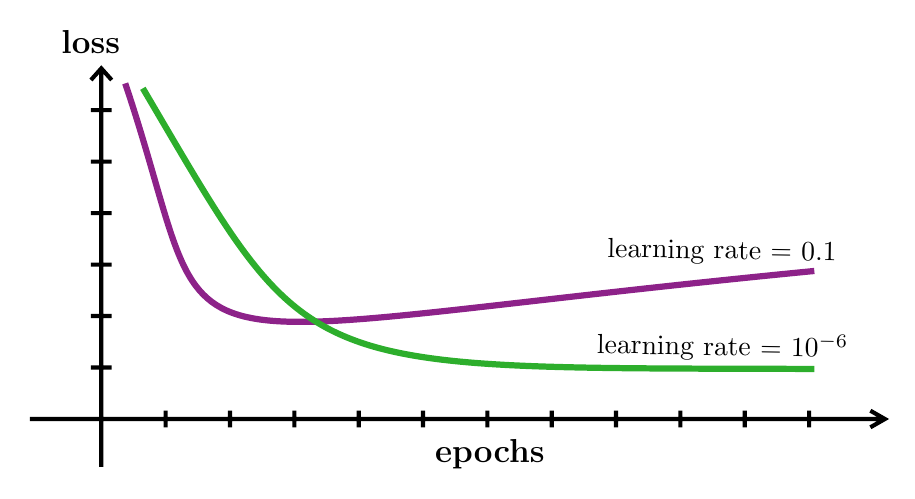
\begin{tikzpicture}[x=0.75pt,y=0.75pt,yscale=-0.8,xscale=1]
%uncomment if require: \path (0,380); %set diagram left start at 0, and has height of 380

%Shape: Axis 2D [id:dp9188601223891106] 
\draw [color={rgb, 255:red, 0; green, 0; blue, 0 }  ,draw opacity=1 ][line width=1.5]  (26,335.65) -- (438,335.65)(60.48,124.5) -- (60.48,364.5) (431,330.65) -- (438,335.65) -- (431,340.65) (55.48,131.5) -- (60.48,124.5) -- (65.48,131.5) (91.48,330.65) -- (91.48,340.65)(122.48,330.65) -- (122.48,340.65)(153.48,330.65) -- (153.48,340.65)(184.48,330.65) -- (184.48,340.65)(215.48,330.65) -- (215.48,340.65)(246.48,330.65) -- (246.48,340.65)(277.48,330.65) -- (277.48,340.65)(308.48,330.65) -- (308.48,340.65)(339.48,330.65) -- (339.48,340.65)(370.48,330.65) -- (370.48,340.65)(401.48,330.65) -- (401.48,340.65)(55.48,304.65) -- (65.48,304.65)(55.48,273.65) -- (65.48,273.65)(55.48,242.65) -- (65.48,242.65)(55.48,211.65) -- (65.48,211.65)(55.48,180.65) -- (65.48,180.65)(55.48,149.65) -- (65.48,149.65) ;
\draw   ;
%Curve Lines [id:da09457620026426827] 
\draw [color={rgb, 255:red, 141; green, 34; blue, 137 }  ,draw opacity=1 ][line width=2.25]    (72,133.5) .. controls (121,316.5) and (66,287.5) .. (404,246.5) ;
%Curve Lines [id:da9690899577583578] 
\draw [color={rgb, 255:red, 45; green, 174; blue, 44 }  ,draw opacity=1 ][line width=2.25]    (80.5,136.5) .. controls (163,311.5) and (151,304.5) .. (404,305.5) ;

% Text Node
\draw (303.19,224.98) node [anchor=north west][inner sep=0.75pt]  [rotate=-0.92] [align=left] {learning rate = $0.1$};
% Text Node
\draw (298.19,280.98) node [anchor=north west][inner sep=0.75pt]  [rotate=-0.92] [align=left] {learning rate = $10^{-6}$};
% Text Node
\draw (220,346.46) node [anchor=north west][inner sep=0.75pt]  [font=\large] [align=left] {\textbf{epochs}};
% Text Node
\draw (40.01,100.31) node [anchor=north west][inner sep=0.75pt]  [font=\large] [align=left] {\textbf{loss}};


\end{tikzpicture}